\documentclass[11pt]{article}

\usepackage{epsf}
\usepackage{epsfig}
\usepackage{url}
\usepackage{6829hw}
\input{macros.tex}

\begin{document}

\newcounter{listcount}
\newcounter{sublistcount}


\handout{H1}{August 23, 2011}{Instructor: Prof. Nick Feamster}
{College of Computing, Georgia Tech}{Problem Set 1: Transit Networks}

%\handout{{\bf Problem Set 1}}{September 10, 2002}

This problem set has three questions, each with several parts.  Answer
them as clearly and concisely as possible.  You may discuss ideas with
others in the class, but your solutions and presentation must be your
own.  Do not look at anyone else's solutions or copy them from
anywhere. (Please refer to the Georgia Tech honor code, posted on the
course Web site).

Turn in your solutions in on {\bf September 20, 2011} by 11:59pm.  {\em
  Please upload your solutions to T-Square.  Other forms of submission
  will not be accepted!}

You are welcome to work with one other partner on this problem if you
want, provided you (1)~work out all the problems yourself; (2)~type up
your own assignment; (3)~list on your assignment hand-in the name of the
person you worked with.

%%%%%%%%%%%%%%%%%%%%%%%%%%%%%%%%%%%%%%%%%%%%%%%%%%%%%%%%%%%%
%\newpage
\section{Understanding BGP From Routing Trace File Analysis}

For this question, you will need to download the Routeviews routing
tables from the resources directory on T-Square.  I have pre-processed
the files from the binary routing table dumps so that they are easier to
parse using the {\tt bgpdump} tool that is available at
\url{http://www.ris.ripe.net/source/bgpdump/}.  

You will need the following files to complete the assignment, which are
available on T-Square and at \url{http://gtnoise.net/classes/cs6250/fall_2011/psets/ps1/}:
\begin{itemize}
\itemsep=-1pt
\item The IPv4 BGP routing table snapshot, {\tt
  rib.20110810.0400.txt.gz}
\item The IPv6 BGP routing table snapshot, {\tt
  rib-v6.20110810.0400.txt.gz}
\item The IPv4 BGP {\em update} logs, {\tt updates-v4.20110810.0400.txt.gz}.
\end{itemize}

The files contain Cisco BGP routing table snapshots, taken at Oregon
Route Views (\url{http://www.routeviews.org/}) in August 2011. ({\em
  Beware:} The text files are pre-processed, but they are quite large.
You should be able to analyze it without uncompressing it using, for
example {\tt bzcat}, or with a script.  Do not attempt to open this file
in a window.)  If you are curious about what other snapshots look like,
you can find daily snapshots at \url{http://archive.routeviews.org/}

\subsection*{IPv4 and IPv6 Routing Table Analysis}

\begin{enumerate}

\item Find the routing table entries for the IPv4 and IPv6 Georgia Tech campus
  networks. 
\setcounter{listcount}{0}
\begin{list}{(\alph{listcount})}{\usecounter{listcount}}

\item  What are the IP prefixes for the Georgia Tech network, and
  how did you find them (list both the IPv4 and IPv6 prefixes)?  Why
  might Georgia Tech have more than one IPv4 prefix?

\item From the routing table file, what is the AS number for Georgia Tech? 

\item What is the IPv4 address of the best next hop from this router to
Georgia Tech's /16 IPv4 prefix?  How does this router know how to reach that
next hop IP 
address?

\item How many IPv4 routes are there to get from this router to Georgia
  Tech?  How many IPv6 routes are there to get from this router to
  Georgia Tech?  

\item Suppose that RouteViews routers prefer routes advertised by
  Internet2 over routes received from the ``commodity'' Internet.  From
  your knowledge of the BGP decision process, what is the best IPv4
  route to Georgia Tech?  Why was this route selected as the best
  route?\footnote{If you're interested, see the L4 notes
%\url{http://www.cisco.com/warp/public/459/25.shtml} 
for an overview of
the BGP decision process.  Note that the process is slightly
vendor-specific.}

\item How many ASes must a packet traverse between the time it
leaves the router and the time that it arrives at Georgia Tech?

\item What are the AS numbers and names of all of Georgia Tech's upstream
  providers for IPv4 connectivity? Which ISPs do each of the above ASes
  correspond to?  Who are the upstream providers for IPv6, and why are
  they not the same?  

\item In paths where Georgia Tech uses Cogent (AS~174) as an upstream,
  the AS path ends with five instances of the same AS number (AS~2637).  Why?
  What is the likely relationship between this AS number and Cogent?

\item Look at all of the routes for which the AS path contains the
  sequence {\tt 10490}.  Look at some of the ASes that appear first in
  those AS paths.  Note that many of them are research networks (e.g, AS
  2152).  Why?  There also appear to be other interesting paths to
  Georgia Tech through AS~10490 (e.g., AS~812, or Rogers Cable).  Do
  some research into Internet2's policies to explain why some of these
  ``non research'' paths may exist to Georgia Tech.
\end{list}


\item Use {\tt traceroute} to measure a route from some machine at Georgia
  Tech to the router at RouteViews that took the snapshot.  Please include the output
  of your traceroute with your problem set.

  Is the sequence of ASes from Georgia Tech to the router the same as the
  reverse route in the trace data?   Why might the reverse path differ?
  (Please list reasons other than the fact that your traceroute was
  performed at a different time as the table snapshot!)

\item Most of the IPv4 prefixes are formatted as {\sf w.x.y.z/m}.  The
  mask field, $m$, specifies the length of the network mask to use when
  matching input destination addresses to entries in the table.
\begin{enumerate}

\item Write down the bit-wise operation to determine whether a
destination address, $A_i$, matches a prefix $A/m$ in the routing
table.  $A_i$ and $A$ are 32 bits each.

\item Many of the prefixes and addresses in the IPv6 table are also
  abbreviated.  Write out the 128-bit version of the following address:
  {\tt 2001:470:0:1a::1}.

\item Find the first ``Class C'' CIDR address in the table (address
  prefix $\geq$ 192.0.0.0) that has a mask length less than 24.  How
  many class C networks does this address correspond to?  What is the
  maximum number of routing table entries that this single CIDR address
  saves?  Why is it that we can only infer the maximum, and not the
  actual, number of addresses that this CIDR address saves?

\item In the table, there are examples of groups of prefixes that have
the same advertised AS path, but show up as separate entries in the
routing table.\footnote{For both parts of this problem, it's sufficient
to find the existence of one AS path that is advertised more than once.
It is {\em not} necessary to find two prefixes for which {\em all}
advertised paths are the same.}

\setcounter{listcount}{0}
\begin{list}{(\roman{listcount})}{\usecounter{listcount}}
\item Provide an example of non-contiguous prefixes (and the
corresponding AS path) for which this is true.  Why might non-contiguous
prefixes have the same AS path?
\item Provide an example of contiguous prefixes (and the corresponding
AS path) for which this is true.  This practice is often called {\em
deaggregation}.  Why might this be done?
\end{list}

\end{enumerate}

\item Look at the data at the IPv4 and IPv6 comparative report, here:
  \url{http://bgp.potaroo.net/v6/v6rpt.html}.  Note that the sizes of
  the respective tables, in terms of number of prefixes, roughly agree
  with the tables you downloaded for this assignment.
\setcounter{listcount}{0}
\begin{list}{(\roman{listcount})}{\usecounter{listcount}}
\item Why is the number of ASes that advertise IPv6 prefixes so much
  less?
\item Give a geographic breakdown, by country, of the locations that
  advertise IPv6 prefixes.  (i.e., what fraction of the IPv6 prefixes
  are advertised by each country)?  Perform this analysis both by (i)
  number of IPv6 routes advertised; (ii) total amount of IPv6 space
  advertised.  
\end{list}

\end{enumerate}

\subsection*{BGP Stability}

BGP is an incremental protocol, sending an update message only when the
route for a destination prefix changes. So, most analysis of BGP updates
must start with a snapshot of the RIB, to know the initial route for
each destination prefix. Use the RIB snapshot of the IPv4 prefixes from
the first part of this assignment to identify the initial set
of destination prefixes. Then analyze the next several hours of
update messages using the BGP update logs to count the number of update
messages for each prefix.

\begin{enumerate}
\item What fraction of IP prefixes experience no update messages? (Count each prefix
equally, independently of what fraction of address space they cover or whether one prefix is
contained inside another.) 
\item What prefix experiences the most updates, and how frequent are they?
\item Plot the probability distribution of the number (or fraction) of updates by prefix.
Choose whether to plot a Cumulative Distribution Function or Complementary CDF, and
either log or linear axes, to highlight the main interesting features of the distribution.
\item Briefly summarize your results and what you learned about BGP
  stability from them.
\end{enumerate}

\section{Understanding IS-IS Using Packet Traces}

Obtain the IS-IS packet traces from the Abilene network for August 21,
2011.  For example, the trace from the Atlanta router is located at
{\url{http://ndb7.net.internet2.edu/isis/ATLA/2011/08/isisd.20110820.gz}}.
Seven of the 11 Abilene backbone routers capture such traces.  

\begin{enumerate}
\item In the trace, list the different types of IS-IS messages that you
  see and the purpose of each message.
\item Look at the LSA packet in the trace from Aug 19, 2011
  20:03:08.866466000  to answer the following
  questions:
\setcounter{listcount}{0}
\begin{list}{(\roman{listcount})}{\usecounter{listcount}}
\item In the IP internal reachability part of the LSA, there is an IP
  prefix, ``IPv4 prefix: 64.57.28.12/31, Metric: 905, Distribution: up,
  no sub-TLVs present''.  What does that prefix refer to, and what is it
  advertising reachability to? 
\item What is the remaining lifetime of this link-state advertisement?
\item List the other /31 prefixes in this LSA and their metrics.
\item What does ``IS Reachability'' mean, as opposed to ``IP Internal
  Reachability''. 
\end{list}
\item Which router advertised this LSA?  When is the next time it
  advertises an LSA that is heard at this router?
\item Suppose that you wanted to design an IS-IS monitoring tool to
  detect failures.  Sketch a rough design for this system.  What would
  messages would you detect, and how?  Be specific about what routers
  you would collect data from and where.
\end{enumerate}


\section{Inferring AS Relationships}

As you know, the Internet is composed of nearly 40,000 distinct origin
ASes that exchange routes to establish global connectivity, and that
business relationships determine which routes are exchanged between each
pair of ASes.  

Recall that one network will re-advertise its customer routes to its
peers and providers, but will not re-advertise routes heard from a peer
to other peers or providers.  With the knowledge of these rules and a
view of a default-free routing table (or multiple tables), one can
deduce relationships between AS pairs based on links that exist in the
AS graph.  

In {\em On Inferring Autonomous System Relationships in the Internet}
(the reading for L4), Lixin Gao observes that, because of these
constraints, AS paths must adhere to one of the following patterns:

\begin{itemize}
\itemsep=-1pt
\item a series of customer-provider links (an {\em uphill path})
\item a series of provider customer links (a {\em downhill path})
\item an uphill path followed by a downhill path
\item an uphill path followed by a peering link
\item an peering edge followed by a downhill path
\item an uphill path followed by a peering link, followed by a downhill
  path
\end{itemize}

This is called the ``valley free'' property of AS paths.  The hard
question, of course, is: where is the ``top of the hill''?  

In this problem, you will implement Gao's algorithm for inferring AS
relationships, using the BGP routing table dump from the first problem
of this problem set.

\setcounter{listcount}{0}
%\begin{list}{(\alph{listcount})}{\usecounter{listcount}}

\begin{enumerate}

\item Why do the provided routing tables only have a single route per
  prefix? 

\item What heuristic does Gao suggest for finding the top of the hill?

\item Produce a Complementary Cumulative Distribution Function (CCDF) of
  AS degree (i.e., plot the fraction of ASes that have an degree of
  $\geq n$, for all $n>0$).  Also include a table of the ``top 10'' ASes
  for degree and the value of their degrees. Do not count a link from an
  AS to itself as an edge.  Also, consider {\em all} AS paths that are
  given in the table, not just the best path for each prefix.

\item For each of the following AS paths, list the transit
relationships inferred for each pair, based on that path.  {\em This is a
two-step process.}

First, for each AS path, note the transit relationships.  For example,
for the path $A B C D$, if $C$ were the AS with the highest degree,
you would write ``Transit relationships: $A\rightarrow B$,
$B\rightarrow C$, $D\rightarrow C$''.  This will give you a list of AS
pairs that have transit relationships.

Once you have scanned all AS paths, you may find that you
have a commutative transit relationship: i.e., $A$ transits $B$ {\em
and} $B$ transits $A$.  This is called a sibling relationship.   For
all pairs in the following paths, note which AS transits for the
other, or if the two pairs have a sibling relationship.

\setcounter{sublistcount}{0}
\begin{list}{(\alph{sublistcount})}{\usecounter{sublistcount}}
\item 7018 3356 22961
\item 31500 3267 3356 2516 2519
\item 701 2914 4641 38345
\item 2914 9318 38091 18313
\item 8492 9002 9318 38091 18313
\end{list}

\item Finding the ``top of the hill'' by using the AS with the highest
degree sometimes produces the wrong answer.  Another way to do this is
to view the AS paths from one vantage point as a directed graph, and
using a reverse pruning algorithm to the AS graph in order to assign
ranks to each AS.

First, leaf nodes of the AS graph are assigned the lowest rank.  Then,
these nodes and their incident edges are removed from the graph.  The
nodes that are leaves in this new graph are assigned the next highest
rank.  The process repeats until the graph is strongly-connected (i.e.,
there are no leaves); each node in the strongly-connected component of
the graph receives the highest rank.  AS relationships are inferred by
comparing rankings from AS graphs as visible from {\em multiple vantage
points}\footnote{You can find the paper that describes this algorithm in
detail at \url{http://www.ieee-infocom.org/2002/papers/594.pdf}.}.

\setcounter{sublistcount}{0}
\begin{list}{(\alph{sublistcount})}{\usecounter{sublistcount}}
\item What are advantages of using this type of ranking scheme over a
power-law based scheme?  What are the disadvantages?
\item Why does this scheme require multiple vantage points to be
effective? 
\end{list}

\end{enumerate}


\section{Emulab: Experience with ARP and OSPF}

{\em Complete this section of the assignment in groups.}

This problem will give you hand-on experience with Layer 2 and Layer 3
protocols, and with setting up network experiments in Emulab.  The
experimental configuration language is based on Tcl, which is the same
as that which is used for {\em ns}, a network simulator.

\subsection*{Setting Up Your Experiment}

\begin{enumerate}
\itemsep=-1pt
\item{\bf Emulab} Go to \url{http://www.emulab.net} and request an
  account. Join project `cs6250', group `cs6250'.  {\em Do this early, as
    I will need to approve your membership!}

\item{\bf Topology Setup.} Write a tcl procedure that takes an integer
  $n$ and creates a dumbell topology as shown in the figure below.  You
  can test your code on emulab or in {\em ns}.  Make all ``edge'' links
  in the topology 100Mbps/10ms duplex links, with DropTail queues, and
  the link between $R_1$ and $R_2$ a 1Mbps/10ms duplex link.  The figure
  has some nodes named ``router'', but in fact all of these should
  simply be Emulab hosts. {\em If you run into resource constraints on
    Emulab, you can create a dumbbell with one node on each side of the
    dumbbell and still complete the assignment.}

\begin{center}
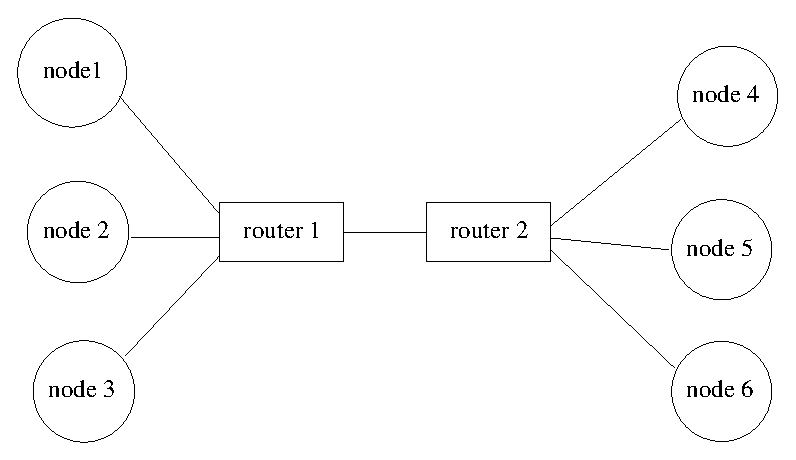
\includegraphics[width=0.5\linewidth]{db}
\end{center}

  {\em Hint:} Reading Emulab and ns documentation will help with this
  problem.

\item {\bf Topology Creation.} Create your topology in Emulab.  You
  can use the Emulab interface to get the DNS names and IP addresses of
  each of the nodes in your topology.  

  You should be also able to {\tt ssh} to the nodes and send pings to
  and from each of the nodes at this point.  We will now experiment on
  the nodes themselves.

\item {\bf Assigning IP addresses to your nodes.} By default, the Emulab
  experiment manager assigns hosts each Ethernet segment with IP
  addresses from distinct subnets; it will then install routing tables
  in the kernel and try to route packets based using the kernel routing
  table.  Since you are doing an experiment that involves constructing a
  layer-2 topology, you will want to remove these routing table entries,
  assign hosts IP addresses from the same subnet, or both.  The
  instructions at
  \url{https://users.emulab.net/trac/emulab/wiki/Nscommands#IPAddressCommands}
  explain how to automate IP address assignment in the experiment script
  itself.  

\end{enumerate}

\subsection*{ARP and Click}

\begin{enumerate}
\itemsep=-1pt
\item{\bf LAN Setup} Put all of the nodes in a large LAN in your
  configuration file.  
  \begin{enumerate}
    \item Log into {\em node1} and print the ARP table (include the
      output in your hand-in).  Ping {\em router1}.  Print the ARP table
      again.  What happened?
    \item What does the ``C'' flag mean in the ARP table?
  \end{enumerate}

\item{\bf Writing Your own Switch} In this part of the problem, you'll
  write the switch table entries yourself using Click.  Fortunately for
  you, Click already has an {\tt EtherSwitch} element, so most of the
  ``hard work'' is done.  You just have to figure out how to set it up!

  \begin{enumerate}
    \item Modify your experiment script so that instead of all the nodes
      being placed on a single LAN, the nodes are simply set up as
      point-to-point links.  You should be able to test this because
      you'll only be able to ping adjacent nodes in the dumbbell
      topology.
    \item Download, compile, and install the Click
      (\url{http://www.read.cs.ucla.edu/click/}) modular
      router on {\em router1} and {\em router2} in your topology.

      {\em Possibly helpful hint:} To save yourself the trouble of
      compiling on the nodes themselves, you can compile on a (possibly
      faster) home machine, and then use emulab's {\tt tb-set-node-os}
      command to install the proper OS on the Emulab node that will run
      your binary.

    \item Install and configure the Click elements on {\em router1} and
      {\em router2} so that all nodes in the topology can ping each
      other.  The {\tt EtherSwitch} element will likely be quite helpful
      for you in this regard; {\tt ListenEtherSwitch} might also be
      helpful, particularly for debugging.
  \end{enumerate}

\item{\bf Quick and Dirty Performance Evaluation}
  \begin{enumerate}
    \itemsep=-1pt
    \item Log into {\em node4} and start a tcpdump that looks for ARP
      packets. 
    \item Log into {\em node1} and begin pinging {\em node4}.
    \item Show the packet trace excerpt containing the ARP query and response.  
    \item Modify your experiment setup so that the interface on {\em
      node4} that faces {\em router2} fails.  Explain what you did to do
      this.  Also give one other way you might have simulated this kind
      of effect.  ({\em Hint:} You can do this manually on the node,
      automatically using Emulab, with Click, etc.).  Reinstate the link
      after you're done with the next part of the problem.
%    \item How long does it take before {\em node1}'s ARP table entry
%      expires? 
    \item How long does it take before {\em node4} begins responding to
      pings after you have reinstated the link? 
  \end{enumerate}

\end{enumerate}

\subsection*{OSPF}

In this part of the problem, you will configure the
Quagga (\url{http://www.quagga.net/}) software router's OSPF module to
connect the nodes in your topology.

\begin{enumerate}
\itemsep=-1pt
\item Uninstall Click, but keep the point-to-point Emulab topology.
  Your topology should now be as before: each node should be able to
  ping its immediate neighbors, but no other nodes in the topology. 
\item Install and configure OSPF on each of the nodes in the topology.
  (If you want to save work, it's fine if you only install OSPF on {\em
  node1}, {\em node4}, {\em router1} and {\em router2}, but you will see
  more of the flooding effects if you install everywhere.  You can also
  save work by using a Perl, Ruby, or Python script to generate your
  configuration.)
\item How often do you see OSPF ``Hello'' messages?  How often do you
  see an LSA message for any single link?
\item Repeat the ``quick and dirty performance evaluation'' above where
  you fail a link in the topology and then bring it back.  How long does
  it take before {\em node1}'s routing table entries reflect that node4
  is ``dead''? 
\end{enumerate}

\end{document}
